\providecommand{\main}{..}
\documentclass[\main/main.tex]{subfiles}

\begin{document}
\graphicspath{{img/}{06_result/img/}}

\chapter{System evaluation}

\section{Whole system overview}
\begin{figure}[H]
    \centering
    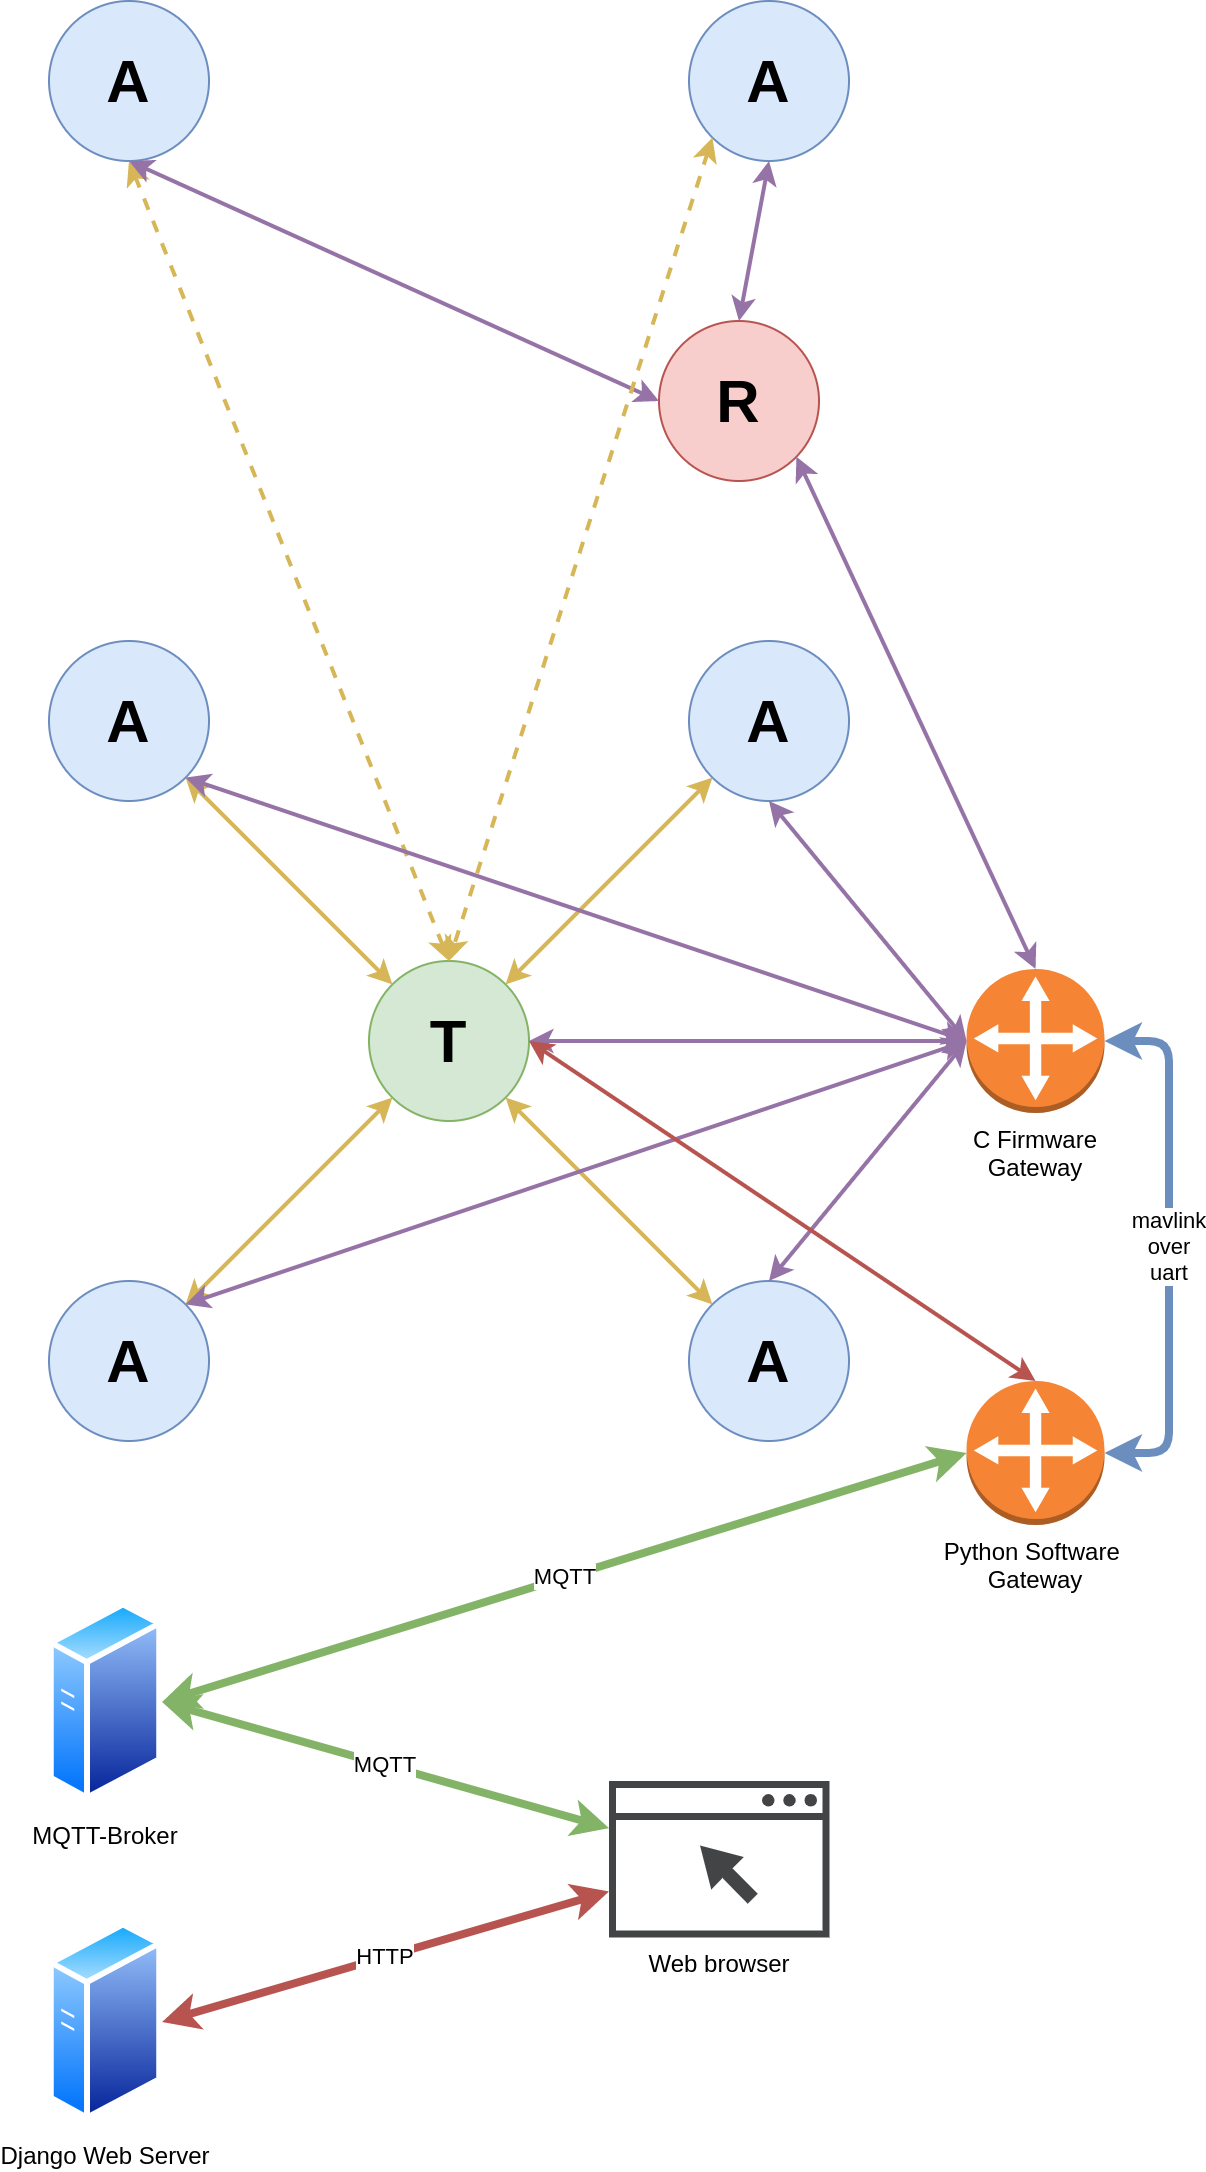
\includegraphics[width=0.8\textwidth]{system_overview.png}
    \caption{Whole system overview}
    \label{fig:system_overview}
\end{figure}
The whole system deployed in this thesis is illustrated in figure \ref{fig:system_overview}. There are two cells in the sample network and one tag located in each cell. Tags and anchors communicate with each other using 802.15.4 protocol over UWB radio. They, however, exchange messages with a gateway through a Bluetooth mesh network. The role of the relay node is to relay Bluetooth mesh messages as the distance between anchors/tags and gateway may longer than the effective communication range of Bluetooth-based devices. The firmware and software part of the gateway internally communicate using MAVLink protocol over a UART connection. The MAVLink frame is then stringified to JSON format and published to an MQTT broker. The control and management system is a web-based application. The Django server provides web service for this application. When receiving an HTTP request from the browser, the server returns an HTML/CSS-based GUI (Graphic User Interface) together with instructions for the browser to connect to the MQTT broker. In this way, the browser subscribes to the right topic. On receiving messages, the browser processes and shows them on the screen in a programmed way. On receiving controls from users, the browser publishes the corresponsive JSON messages to the indicated topic which has been already subscribed by the gateway. The gateway then passes such messages to the mesh network.

\section{Evaluation}

In the experimental, the localization error is calculated follow equation \ref{eqn:root_mean_square}.
\begin{equation}
    e_{RMS} = \sqrt{\frac{1}{n} \sum_{k=1}^{n} ((x_k-x_{kg})^2 + (y_k-y_{kg})^2 + (z_k-z_{kg})^2)}
    \label{eqn:root_mean_square}
\end{equation}

\subsection{Preparation}
This subsection provides images to illustrate the experimental setup used to evaluate the proposed localization system. The logical configuration of the system has been given in figure \ref{fig:system_overview}. The physical placement of devices is represented in figure \ref{fig:physical placement of devices}.

\begin{figure}[H]
    \begin{minipage}[t]{\textwidth}       
        \centering
        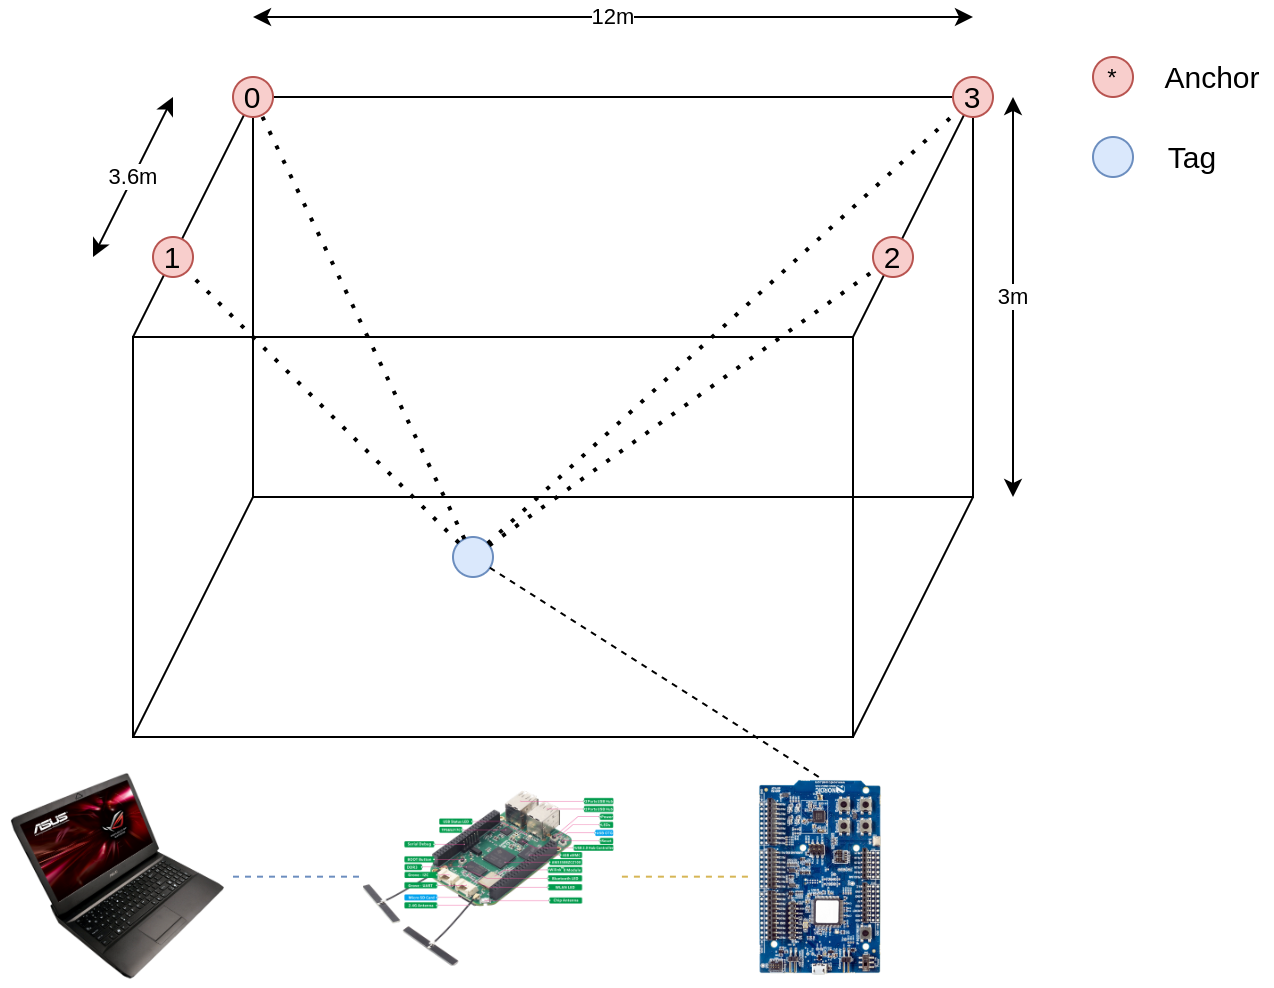
\includegraphics[width=0.9\textwidth]{system_overview_phy.png}
    \end{minipage}
    \caption{Physical placement of devices}
    \label{fig:physical placement of devices}
\end{figure}
The actual placement of device is shown in figure:..., ..., ...

The control and management interface for the experiment is shown in figure \ref{fig:proposed_rms_error}.
\begin{figure}[H]   
    \centering
    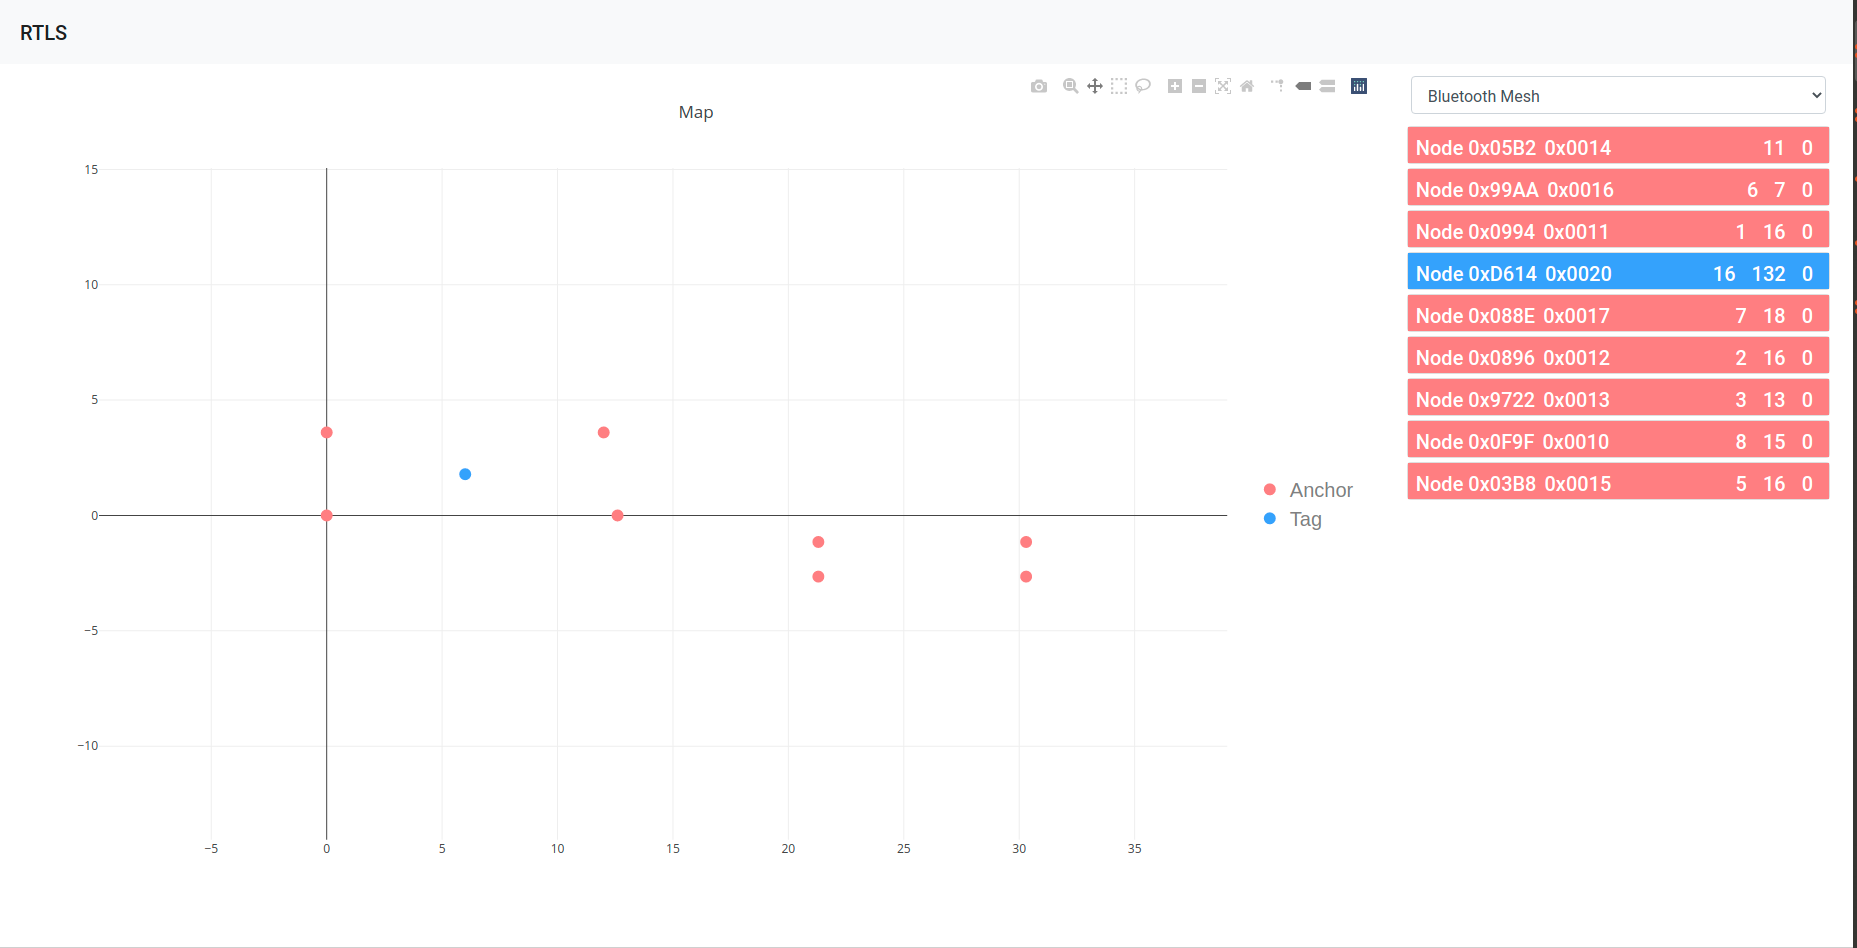
\includegraphics[width=1\textwidth]{result_gui.png}
    \caption{Indoor localization system GUI}
    \label{fig:result_gui}
\end{figure}

\subsection{Result}

Table \ref{table:vendor_rms_error} provides RMS errors of the vendor reference system related to the position $(x,y)$. These errors are also graphically illustrated in \ref{fig:vendor_rms_error}.

Table \ref{table:proposed_rms_error} provides RMS errors of the proposed system related to the position $(x,y)$. These errors are also graphically illustrated in \ref{fig:proposed_rms_error}.

All experiments are done with $z=3$.  

\begin{table}[ht]
    \centering
    \begin{tabular}{|c|>{\centering\arraybackslash}p{2cm}|>{\centering\arraybackslash}p{2cm}|>{\centering\arraybackslash}p{2cm}|}
    \hline
    \backslashbox{y(m)}{x(m)}  &  3 & 7 & 10 \\ \hline
    0 &  0.2 &  0.28 &  0.25  \\ \hline
    2 &  0.14 &  0.13 &  0.18  \\ \hline
    4 &  0.22 &  0.19 &  0.27  \\ \hline
    \end{tabular}
    \caption{Vendor system error}
    \label{table:vendor_rms_error}
\end{table}

\begin{table}[H]
    \centering
    \begin{tabular}{|c|>{\centering\arraybackslash}p{2cm}|>{\centering\arraybackslash}p{2cm}|>{\centering\arraybackslash}p{2cm}|>{\centering\arraybackslash}p{2cm}|}
    \hline
    \backslashbox{y(m)}{x(m)}  &  1.2 & 4.8 & 9.6 & 10.8 \\ \hline
    0.6 &  0.10 & 0.28&  0.13 &  0.12  \\ \hline
    1.2 &  0.13 & 0.18&  0.17 &  0.16  \\ \hline
    2.4 &  0.09 & 0.10&  0.11 &  0.22  \\ \hline
    \end{tabular}
    \caption{Proposed system error}
    \label{table:proposed_rms_error}
\end{table}

\begin{figure}[H]
    \begin{minipage}[t]{\textwidth}       
        \centering
        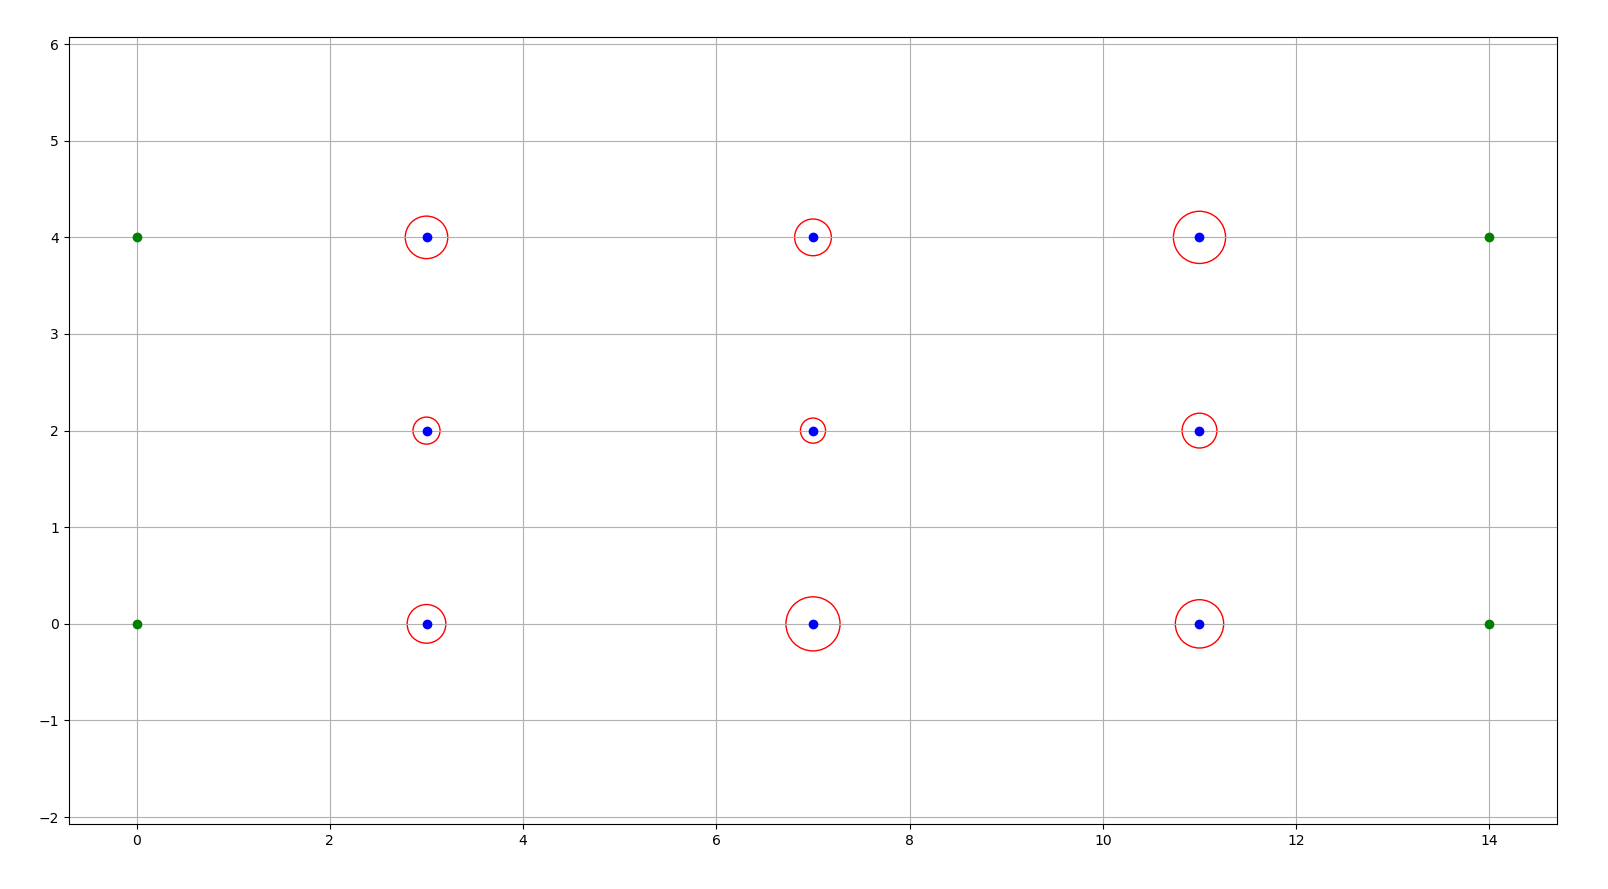
\includegraphics[width=0.9\textwidth]{rms_error}
    \end{minipage}
    \caption{Vendor system error}
    \label{fig:vendor_rms_error}
\end{figure}

\begin{figure}[H]     
    \centering
    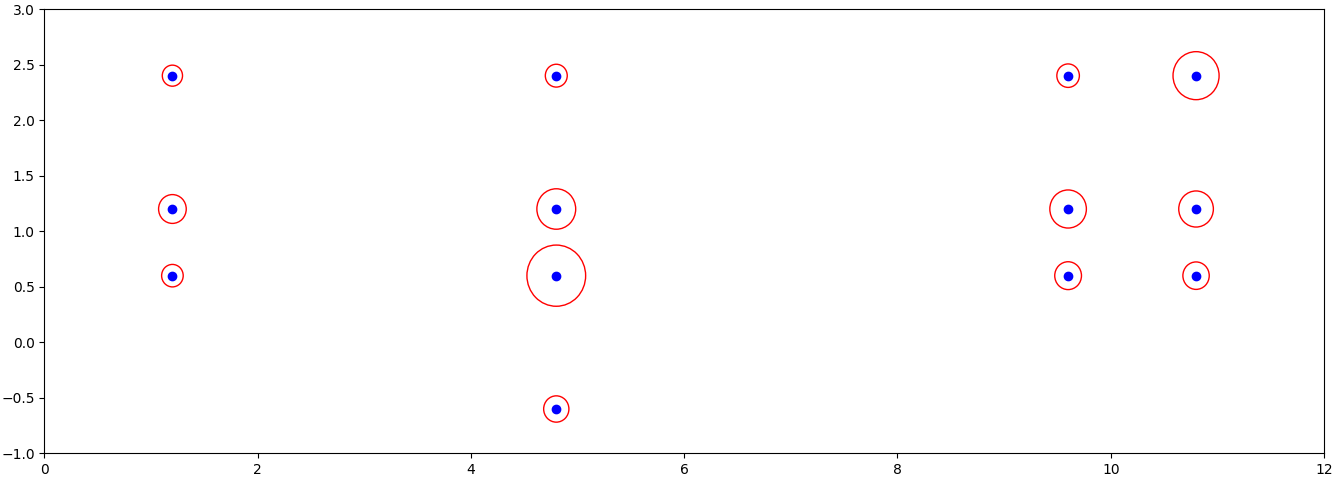
\includegraphics[width=1\textwidth]{result.png}
    \caption{Proposed system error}
    \label{fig:proposed_rms_error}
\end{figure}

\section{Conclusion}
Using experimental results obtained from a decimeter-accuracy 3D indoor localization system, we conclude that the proposed system has a similar performance to the reference system given by the DecaWave while provides a better IoT service (Bluetooth mesh instead of normal Bluetooth Low Energy) which reduce the price of the entire system.
\end{document}